\section{Sigmoid Neurons}

\begin{itemize}
  \item \underline{Anforderung:} Eine kleine Änderung in den Weights/Bias-Werten führt nur zu einer kleinen Änderung in der Ausgabe
  \item $\Rightarrow$ Perceptrons sind dafür nicht geeignet, da sie nur flippen können
  \item \emph{Sigmoid Neurons}:
  \begin{itemize}
    \item \underline{Eingaben:} $x_1, x_2, \ldots, x_n \in [0, 1]$
    \item \underline{Ausgabe:} $\sigma(w \cdot x + b) = \sigma(z) = \frac{1}{1+e^{-z}}$
    \item \underline{Ähnlichkeit:} $z \rightarrow \infty \Rightarrow \sigma(z) \approx 1$ und $z \rightarrow - \infty \Rightarrow \sigma(z) \approx 0$
  \end{itemize}
\end{itemize}

\begin{center}
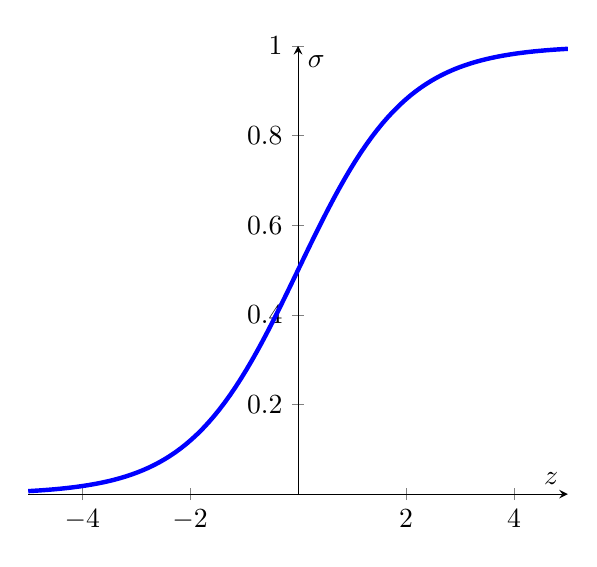
\begin{tikzpicture}
  \begin{axis}[
      axis lines=middle,
      xmax=5,
      xmin=-5,
      ymin=0,
      ymax=1,
      xlabel={$z$},
      ylabel={$\sigma$},
    ]
    \addplot [samples=100, ultra thick, blue] {1/(1+exp(-x))};
  \end{axis}
\end{tikzpicture}
\end{center}

\begin{itemize}
  \item \textbf{Beispiel:} Schrifterkennung
  \begin{itemize}
    \item \underline{Eingabe:} 28 Pixel $\times$ 28 Pixel = 784 Neuronen mit Intensität $\in [0,1]$
    \item \underline{Ausgabe:} 10 Neuronen, die die Wahrscheinlichkeiten beschreiben, dass das Bild die entsprechende Zahl zeigt, d.h.\ $\text{Output} > 0.5$
    \item \underline{Ziel:} approximiere die Funktion $y(x)$, die die Trainingsdaten beschreibt, d.h.\ $y(x) = {(1, 0, 0, 0, 0, 0, 0, 0, 0, 0)}^T$ für ein Bild $x$ mit einer Null, usw.
    \item \underline{Methode:} minimiere Kostenfunktion $C(w,b) = \frac{1}{2n} \sum_x || y(x) - a(x) ||^2$, wobei $a(x)$ der Output des neuronalen Netzes bei Input $x$ ist
  \end{itemize}
\end{itemize}

\subsection{Gradient descent}

\begin{itemize}
  \item \underline{Ziel:} Lösung des Minimierungsproblems $C(v) = C(v_1, v_2, \ldots, v_n)$
  \item \underline{Lösung:}
  \begin{itemize}
    \item definiere den Gradienten $\nabla C  = {(\frac{\partial C}{\partial v_1}, \frac{\partial C}{\partial v_2}, \ldots, \frac{\partial C}{\partial v_n})}^T$ von $C$ aus den partiellen Ableitungen $\frac{\partial C}{\partial v_i}$ von $C$
    \item $\Rightarrow$ $\Delta C \approx \nabla  C \cdot \Delta v$
    \item wähle $\Delta v = - \eta \nabla C$, dann gilt $\Delta C \approx - \eta \nabla C \cdot \nabla C  = - \eta ||\nabla C||^2$ \todo{warum noch mal?}
    \begin{itemize}
      \item $\eta$ wird das \emph{Lerntempo} (engl. \emph{learning rate}) genannt
      \item da $||\nabla C||^2 \geq 0$ folgt, dass $\Delta C \leq 0$ für alle $\eta \in \mathbb{R}^+$
      \item wähle $\eta$ so, dass wir nicht zu langsam lernen, aber dennoch eine gute Approximation erhalten
    \end{itemize}
  \end{itemize}
\end{itemize}

\subsubsection{Gradient descent in neuronalen Netzen}

\begin{itemize}
  \item $\nabla C$ besteht aus partiellen Ableitungen der Komponenten $w_k$ und $b_l$
  \item \underline{Problem:} $\nabla C$ wird berechnet aus dem Mittelwert der Gradienten $\nabla C_x = \frac{1}{2}||y(x)-a(x)||^2$ für alle Trainingsdaten $x$ $\Rightarrow$ berechnungsintensiv
  \item \underline{Lösung:} \emph{Stochastic gradient descent}
  \begin{itemize}
    \item \underline{Idee:} berechne $\nabla C$ aus einer kleinen Anzahl $m$ zufällig gewählter Trainingsdaten $X_1, X_2, \ldots, X_m$
    \item vorausgesetzt $m$ ist groß genug, dann gilt $\frac{1}{m} \sum_{i=1}^m \nabla C_{X_i} \approx \frac{1}{n} \sum_x \nabla C_x = \nabla C$
  \end{itemize}
\end{itemize}
